\begin{filecontents}[overwrite,noheader]{tufte-common-local-before-hyperref.tex}
\usepackage{graphicx}
  \setkeys{Gin}{width=\linewidth,totalheight=\textheight,keepaspectratio}
  \graphicspath{{graphics/}}
\usepackage{booktabs}
\usepackage{multicol}
\usepackage{fancyvrb}
  \fvset{fontsize=\normalsize}
\usepackage{minted-code}
\usepackage{xspace}
\usepackage{amsmath}
\usepackage{siunitx}
\usepackage{makeidx}\makeindex
\usepackage[utf8]{inputenc}
\usepackage[ngerman]{babel}
\babelprovide[hyphenrules=ngerman-x-latest]{ngerman}
\end{filecontents}

\PassOptionsToPackage{style=authoryear,backend=biber}{biblatex}

\documentclass[%
  justified,
  notoc,
  hyperref]{xtufte-book}

\usepackage{c-kurs}

\title{C/C++-Kurs für Kinder ab der 5. Klasse}
\author{Jürgen ``George'' Sawinski}
% \publisher{}

\addbibresource{c-kurs.bib}

\begin{document} 
%%%%%%%%%%%%%%%%%%%%%%%%%%%%%%%%%%%%%%%%%%%%%%%%%%%%%%%%%%%%%%%%%%%%%%%%%%%%%%%
\frontmatter

\maketitle

%%%%%%%%%%%%%%%%%%%%%%%%%%%%%%%%%%%%%%%%%%%%%%%%%%%%%%%%%%%%%%%%%%%%%%%%%%%%%%%
\newpage
\begin{fullwidth}
~\vfill
\thispagestyle{empty}
\setlength{\parindent}{0pt}
\setlength{\parskip}{\baselineskip}
Copyright \copyright\ \the\year\ \thanklessauthor

\par\smallcaps{Veröffentlicht vom Autor}

\par\url{https://github.com/jsawinski/twin-c-course}

\par Licensed under the MIT License

\noindent
Copyright (c) 2026 Jürgen ``George'' Sawinski

\noindent
Permission is hereby granted, free of charge, to any person obtaining a copy
of this software and associated documentation files (the ``Software''), to deal
in the Software without restriction, including without limitation the rights
to use, copy, modify, merge, publish, distribute, sublicense, and/or sell
copies of the Software, and to permit persons to whom the Software is
furnished to do so, subject to the following conditions:

\noindent
The above copyright notice and this permission notice shall be included in all
copies or substantial portions of the Software.

\noindent
THE SOFTWARE IS PROVIDED ``AS IS'', WITHOUT WARRANTY OF ANY KIND, EXPRESS OR
IMPLIED, INCLUDING BUT NOT LIMITED TO THE WARRANTIES OF MERCHANTABILITY,
FITNESS FOR A PARTICULAR PURPOSE AND NONINFRINGEMENT. IN NO EVENT SHALL THE
AUTHORS OR COPYRIGHT HOLDERS BE LIABLE FOR ANY CLAIM, DAMAGES OR OTHER
LIABILITY, WHETHER IN AN ACTION OF CONTRACT, TORT OR OTHERWISE, ARISING FROM,
OUT OF OR IN CONNECTION WITH THE SOFTWARE OR THE USE OR OTHER DEALINGS IN THE
SOFTWARE.

% Hiermit wird jeder Person, die eine Kopie dieser Software und der zugehörigen
% Dokumentationsdateien (die ``Software'') erhält, kostenlos die Erlaubnis erteilt,
% die Software ohne Einschränkung zu nutzen, einschließlich und ohne Einschränkung
% der Rechte zur Nutzung, Vervielfältigung, Bearbeitung, Zusammenführung,
% Veröffentlichung, Verbreitung, Unterlizenzierung und/oder zum Verkauf von
% Kopien der Software, und Personen, denen die Software zur Verfügung gestellt
% wird, dies unter den folgenden Bedingungen zu gestatten:

% Der obige Urheberrechtsvermerk und dieser Genehmigungsvermerk müssen in allen
% Kopien oder wesentlichen Teilen der Software enthalten sein.

% DIE SOFTWARE WIRD ``WIE BESEHEN'' BEREITGESTELLT, OHNE JEGLICHE GEWÄHRLEISTUNG,
% AUSDRÜCKLICH ODER STILLSCHWEIGEND, EINSCHLIESSLICH, ABER NICHT BESCHRÄNKT AUF
% DIE GEWÄHRLEISTUNG DER MARKTGÄNGIGKEIT, DER EIGNUNG FÜR EINEN BESTIMMTEN ZWECK
% UND DER NICHTVERLETZUNG VON RECHTEN DRITTER. IN KEINEM FALL SIND DIE AUTOREN
% ODER RECHTSINHABER FÜR ANSPRÜCHE, SCHÄDEN ODER ANDERE VERPFLICHTUNGEN HAFTBAR,
% OB IN EINEM VERTRAGS- ODER DELIKTSVERFAHREN ODER ANDERWEITIG, DIE AUS DER
% NUTZUNG DER SOFTWARE ODER IN VERBINDUNG MIT DER NUTZUNG DER SOFTWARE ENTSTEHEN.

% % \par\textit{First printing, \monthyear}
% \small\textit{%
% Die Übersetzung der MIT-Lizenz in die deutsche Sprache ist nicht rechtsverbindlich.\\
% Im Zweifel ist die englische Version maßgeblich.}
\end{fullwidth}

%%%%%%%%%%%%%%%%%%%%%%%%%%%%%%%%%%%%%%%%%%%%%%%%%%%%%%%%%%%%%%%%%%%%%%%%%%%%%%%
% Epilog
\newpage
\par\noindent
Dieser Kurs ist gedacht für Kinder ab Ende der Grundschule (ca. 5. Klasse), 
die Begeisterung für Mathematik und Computer mitbringen und den Drang haben, 
programmieren zu lernen.

Der erste Teil des Kurses beschäftigt sich damit, alle grundlegenden Kenntnisse zu erwerben, um eine Konsolen-basierte Regensimulation in C zu programmieren, was auch mathematische und physikalische Grundlagen beinhaltet.

Der zweite Teil des Kurses wird das Ziel haben, das Spiel Tetris® in C++ umzusetzen, wobei das Hauptaugenmerk dabei auf die Grundlagen Objekt-orientierter Programmierung gelegt wird.

%%%%%%%%%%%%%%%%%%%%%%%%%%%%%%%%%%%%%%%%%%%%%%%%%%%%%%%%%%%%%%%%%%%%%%%%%%%%%%%
\tableofcontents

%%%%%%%%%%%%%%%%%%%%%%%%%%%%%%%%%%%%%%%%%%%%%%%%%%%%%%%%%%%%%%%%%%%%%%%%%%%%%%%
\newpage
\section*{Vorwort}

Dieser Kurs ist aus der gemeinsamen Arbeit des Autors mit seinen Söhnen entstanden.
Die Idee, einen C/C++-Kurs für Kinder zu schreiben, kam von den Jungs selbst,
die unbedingt programmieren lernen wollten um ihre eigenen Spiele zu entwickeln
zu können. 

Die Mitschrift ist in erster Linie für Kinder gedacht, die den Kurs mit einer 
Begleitperson zusammen durchlaufen und dient als Leitfaden sowie als 
Nachschlagewerk für die behandelten Themen. 

Der Autor hat die Inhalte erarbeitet, erklärt und in LaTeX festgehalten.
Bei der Strukturierung des Materials und der Erstellung einiger LaTeX-Makros
wurde er durch KI-gestützte Werkzeuge (\textbf{DeepSeek} und \textbf{GitHub Copilot}) 
unterstützt.

DeepSeek lieferte Vorschläge zur Gliederung, zur didaktischen Aufbereitung
und zu technischen Umsetzungen in LaTeX. Github Copilot wurde beim Schreiben von 
LaTeX-Code und bei der Erstellung von C/C++-Codebeispielen eingesetzt. Alle 
Vorschläge wurden vom Autor geprüft, angepasst und auf die Bedürfnisse seiner 
Kinder zugeschnitten.

\textit{-- Jürgen ``George'' Sawinski, \today}

\vspace{1cm}

%%%%%%%%%%%%%%%%%%%%%%%%%%%%%%%%%%%%%%%%%%%%%%%%%%%%%%%%%%%%%%%%%%%%%%%%%%%%%%%
\section*{Lizenz und Haftungsausschluss}

Alle Inhalte dieses Kurses wurden vom Autor selbst erstellt und sind, 
soweit nicht anders gekennzeichnet, frei von urheberrechtlich geschützten 
Materialien Dritter. Die Beispiele und Übungen sind so gestaltet, dass sie 
die Lernziele unterstützen und den Kindern helfen, die Konzepte zu verstehen 
und anzuwenden.

Dieses Werk wird unter der \textbf{MIT-Lizenz} veröffentlicht. 
Das bedeutet: Ihr dürft es kopieren, verändern, weitergeben und 
für eigene Zwecke nutzen — auch kommerziell. Die einzige Bedingung ist, 
dass der Autor (Jürgen ``George'' Sawinski) in der Quellenangabe genannt wird.

\textbf{Haftungsausschluss:} 
Dieser Kurs wurde mit größter Sorgfalt erstellt. Dennoch übernimmt der Autor 
keine Gewähr für die Richtigkeit, Vollständigkeit oder Aktualität der Inhalte. 
Die Nutzung der Inhalte erfolgt auf eigene Verantwortung. Der Autor haftet nicht 
für Schäden, die aus der Nutzung oder der Unfähigkeit zur Nutzung der Inhalte 
entstehen.

\vspace{1cm}
\noindent
\textbf{Projekt-Webseite:} \url{https://github.com/jsawinski/twin-c-course}


\mainmatter

%%%%%%%%%%%%%%%%%%%%%%%%%%%%%%%%%%%%%%%%%%%%%%%%%%%%%%%%%%%%%%%%%%%%%%%%%%%%%%%
%%%%%%%%%%%%%%%%%%%%%%%%%%%%%%%%%%%%%%%%%%%%%%%%%%%%%%%%%%%%%%%%%%%%%%%%%%%%%%%
%%%%%%%%%%%%%%%%%%%%%%%%%%%%%%%%%%%%%%%%%%%%%%%%%%%%%%%%%%%%%%%%%%%%%%%%%%%%%%%
\part{Die Programmiersprache C}

%%%%%%%%%%%%%%%%%%%%%%%%%%%%%%%%%%%%%%%%%%%%%%%%%%%%%%%%%%%%%%%%%%%%%%%%%%%%%%%
%%%%%%%%%%%%%%%%%%%%%%%%%%%%%%%%%%%%%%%%%%%%%%%%%%%%%%%%%%%%%%%%%%%%%%%%%%%%%%%
\chapter{Ein paar Grundlagen}
\label{sec:grundlagen}
\section{Das Binärsystem}
\label{sec:grundlagen:binärsystem}

Computer rechnen im sogenannten Binärsystem, sie kennen nur 0 und 1. Um größere Zahlen darstellen zu können, werden mehrere dieser Nullen und Einsen, genannt ``\textbf{Bit}'' aneinandergereit. Am gebräuchlichsten dabei ist das ``\textbf{Byte}'' (siehe Abb.~\ref{fig:byte-bits}), das aus 8 Bit besteht.

\begin{marginfigure}
  \centering
  \begin{tikzpicture}[
      cell/.style={
          draw,
          rectangle,
          minimum width=0.5cm,
          minimum height=0.5cm,
          font=\ttfamily,
          outer sep=0pt,          % Kein Abstand zwischen Zellen
          anchor=base,
      },
      xscale = 0.5,
  ]

  % Bit-Positionen (0 bis 7) nebeneinander
  \foreach \i in {0,1,...,7} {
      \node[cell] at (7-\i,0) (bit\i) {\i};
  }

  % Border around entire byte
  \node[draw=black, thick, inner sep=4pt, fit=(bit0)(bit7)] (bytebox) {};

  % Etikett "Bit" darüber
  \node[font=\sffamily, left=0.1cm of bytebox] {\textbf{Bit}};

  \end{tikzpicture}
  \caption{Ein Byte mit den Bit-Positionen 0 bis 7.}
  \label{fig:byte-bits}
\end{marginfigure}

\noindent
Jedem Bit wird nun ein Wert zugeordnet. Das erfolgt mathematisch gemäß:
\begin{equation*}
  2^b
\end{equation*}
wobei $b$ die Nummer des Bits ist. Das ist die sogenannte ``Potenz'', eine mathematische Operation\footnote{%
  In der Schule habt Ihr wahrscheinlich den Begriff der Grundrechenarten (oder Grundrechnungsarten) kennengelernt. Der Begriff ``Operation'' bedeutet \emph{Ausführungshandlung}, also ein Vorgang, bei dem aus einem oder mehreren Werten ein neuer Wert berechnet wird - oder in anderen Worten eine \emph{Rechnungsart}. Die \textbf{Zeichen}, die diese Operationen beschreiben (wie \texttt{+}, \texttt{-}, \texttt{\&}, \texttt{|}), nennt man \textbf{Operatoren}. Die Werte, mit denen eine Operation arbeitet, heißen \textbf{Operanden}. Zum Beispiel sind die Grundrechenarten, die Ihr in der Schule gelernt habt, also Addition, Subtraktion, Multiplikation und Division (Plus, Minus, Mal, Geteilt), sogenannte \textbf{arithmetische Operationen}.}
die sagt, wie oft eine Zahl mit sich selbst multipliziert wird. In diesem Fall wird die ``2'' $b$-mal mit sich selbst multipliziert, zum Beispiel:
\begin{align*}
  2^1 &= 2              &= 2\\
  2^2 &= 2\cdot2        &= 4\\
  2^3 &= 2\cdot2\cdot2  &= 8
\end{align*}
Interessant ist nun die Frage, was $2^0$ ist. Wenn Ihr genau hinschaut, dann merkt Ihr, dass, um in die nächste Zeile zu kommen, Ihr das Ergebnis mit $2$ multipliziern müsst. Umgekehrt genauso: um in die vorhergehende Zeile zu kommen, muss man durch $2$ teilen. Wenn also $2^1$ zwei ist und man, um zu $2^0$ zu kommen durch zwei Teilen muss, dann ergibt sich
\begin{equation*}
  2^0 = 1\,.
\end{equation*}
Übrigens, jede Zahl hoch $0$ hat als Ergebnis die $1$ (wir kommen später darauf zurück).\footnote{%
  Es gibt ein Ausnahme und das ist $0^0$. Wenn Ihr diese Rechnung auf dem Computer ausführt, dann erhaltet Ihr als Ergebnis höchstwahrscheinlich auch die $1$. Die Mathematik dahinter kommt allerdings nicht zu einem eindeutigen Ergebnis.}

Um auf das \textbf{Byte} zurückzukommen, heißt dass, dass den \textbf{Bits} jeweils die Werte 1 bis 128 zugeordnet sind (siehe Abb.~\ref{fig:byte-values}).

\begin{figure}[h]
  \centering
  \begin{tikzpicture}[
      cell/.style={
          draw,
          rectangle,
          minimum width=0.8cm,
          minimum height=0.8cm,
          font=\ttfamily\large,
          outer sep=0pt,          % Kein Abstand zwischen Zellen
          anchor=base,
      }
  ]

  % Zeile 1: Bit-Positionen (0 bis 7)
  \foreach \i in {0,1,...,7} {
      \node[cell] at (7-\i,0) (bit\i) {\i};
  }

  % Zeile 2: Werte (1, 2, 4, 8, 16, 32, 64, 128)
  \foreach \i in {0,1,...,7} {
      \node[cell] at (7-\i,-1.2) (val\i) {\pgfmathparse{int(2^\i)}\pgfmathresult};
  }

  % Border around
  \node[draw=black, thick, inner sep=4pt, fit=(bit0)(bit7)] (bytebox) {};
  \node[draw=black, thick, inner sep=4pt, fit=(val0)(val7)] (valbox) {};


  % Etiketten "Bit" und "Wert" darüber
  \node[font=\sffamily, left=0.1cm of bytebox] {\textbf{Bit}};
  \node[font=\sffamily, left=0.1cm of valbox] {\textbf{Wert}};

  \end{tikzpicture}
  \caption{Ein Byte mit Bit-Positionen und den zugehörigen Werten ($2^b$).}
  \label{fig:byte-values}
\end{figure}

\noindent
Damit können wir nun die Zahlen 0 bis 255 darstellen, z.B.:
\begin{align*}
  00000000 &\rightarrow 0\,, \\
  00000011 &\rightarrow 3\,, \\
  01011000 &\rightarrow 88\,, \\
  11111111 &\rightarrow 255\,.
\end{align*}
Das Addieren funktioniert nun genauso, wie Ihr es aus der Schule, in der natürlich das Zehnersystem verwendet wird, gelernt habt. Beispiel:
\begin{lstlisting}
      00100111       39
    + 00000110     +  6
          11         1     (Übertrag)
     ---------      ---
      00101101       45
\end{lstlisting}
Entsprechend lässt sich auch die Multiplikation durchführen:
\begin{lstlisting}
      00001010·00101010 =     10·42
               ..|.|.|.
        00000000.|.|.|.
         00000000|.|.|.
          00001010.|.|.
           00000000|.|.
            00001010.|.
             00000000|.
              00001010.
               00000000
               1 1             (Übertrag)
        ---------------
              110100100        420
\end{lstlisting}
Wenn Ihr genau hinseht, dann bemerkt Ihr, dass wir zwei Bytes multipliziert haben, aber das Ergebnis benötigt 9 Bits, also ein Bit mehr als ein Byte. Das führt zu dem Problem, dass, wenn Ihr auf einem Computer diese Multiplikation durchführt, das höchste Bit (die letzte ``1'' links) abgeschnitten wird und das Ergebnis, dass der Computer euch liefert, $164$ ist. Das gleiche passiert bei einem Byte, wenn Ihr zu $255$ die $1$ dazuzählt, das Ergebnis ist $0$ (in der Fachsprache als \textbf{Überlauf} bezeichnet).

Computer können auch negative Zahlen darstellen. Dazu nützt man aus, dass, wenn $255 + 1$ zum Ergebnis $0$ hat, dann hat $0-1$ als Ergebnis $-1$, binär also 11111111. Dies nennt man das ``Zweierkomplement'' (den Begriff müsst Ihr euch natürlich nicht merken). Wichtig ist: das höchste Bit zeigt, dass es sich um eine negative Zahl handelt. Damit können dann mit einem Byte die Zahlen -128 bis 127 dargestellt werden:
\begin{lstlisting}
    10000000        -128
    10000001        -127
    ...
    11111111        -  1
    00000000           0
    00000001           1
    ...
    01111111         127
\end{lstlisting}
Wie wird nun aus einer positiven Zahl eine Negative? Das passiert, indem man alle Bits invertiert (das heißt, aus 0 wird 1 und aus 1 eine 0) und 1 addiert:
\begin{lstlisting}
(-127)  10000001  ->  01111110
                     +00000001
                      --------
                      01111111     (127)
\end{lstlisting}
Das funktioniert auch umgekehrt, also aus einer negativen Zahl eine positive zu machen:
\begin{lstlisting}
(127)   01111111  ->  10000000
                     +00000001
                      --------
                      10000001     (-127)
\end{lstlisting}
Das Interessante an diesem ``Zweierkomplement'' ist nun, dass man, z.B. eine Addition mit genau der gleichen Methode wie bei positiven Zahlen durchführen kann. Beispiel:
\begin{lstlisting}
    00000101       5
  + 11111111      -1
    1111111       (Übertrag)
  -----------
    00000100       4
\end{lstlisting}
Und in der Tat werden im Prozessor des Computers Addition und Subtraktion von positiven und negativen Zahlen auf genau diese Weise durchgeführt, ohne dass der Prozessor speziell zwischen positiven und negativen Zahlen unterscheiden muss. Im nächsten Abschnitt lernt Ihr nun die Grundelemente, aus denen ein Computer, sowie genau diese Rechenoperationen, aufgebaut sind.
\section{Logikgatter — die Bausteine des Prozessors}
\label{sec:grundlagen:logikgatter}

Bevor wir verstehen, wie Computer rechnen, müssen wir wissen, woraus sie gebaut sind.
Das Herzstück eines Computers ist der Prozessor (die CPU). Er besteht aus vielen
kleinen Schaltungen, die mit nur zwei Zuständen arbeiten: \textbf{0} und \textbf{1}.

Diese Schaltungen nennt man \textbf{Logikgatter}. Die wichtigsten sind:

\begin{description}
  \item[UND-Gatter (AND)]\hfill\\
    Das UND-Gatter liefert nur dann eine 1, wenn beide Eingänge 1 sind.
    \begin{center}
    \begin{tabular}{c|c|c}
    A & B & A AND B \\
    \hline
    0 & 0 & 0 \\
    0 & 1 & 0 \\
    1 & 0 & 0 \\
    1 & 1 & 1 \\
    \end{tabular}
    \end{center}

  \item[ODER-Gatter (OR)]\hfill\\
    Das ODER-Gatter liefert eine 1, wenn mindestens einer der Eingänge 1 ist.
    \begin{center}
    \begin{tabular}{c|c|c}
    A & B & A OR B \\
    \hline
    0 & 0 & 0 \\
    0 & 1 & 1 \\
    1 & 0 & 1 \\
    1 & 1 & 1 \\
    \end{tabular}
    \end{center}

  \item[XOR-Gatter (exklusives ODER)]\hfill\\
    Das XOR-Gatter liefert eine 1, wenn genau einer der Eingänge 1 ist.
    \begin{center}
    \begin{tabular}{c|c|c}
    A & B & A XOR B \\
    \hline
    0 & 0 & 0 \\
    0 & 1 & 1 \\
    1 & 0 & 1 \\
    1 & 1 & 0 \\
    \end{tabular}
    \end{center}

  \item[NICHT-Gatter (NOT)]\hfill\\
    Das NOT-Gatter invertiert den Eingang: aus 0 wird 1, aus 1 wird 0.
    \begin{center}
    \begin{tabular}{c|c}
    A & NOT A \\
    \hline
    0 & 1 \\
    1 & 0 \\
    \end{tabular}
    \end{center}
\end{description}

Aus diesen einfachen Gattern kann man alles bauen – sogar eine Addition!
% \begin{exercise}
% ...
% \end{exercise}
\section{Bitweise Operationen in C}
\label{sec:grundlagen:bitweise-operationen}

In der Programmiersprache C könnt ihr diese Logikgatter direkt benutzen.
Die Operatoren dafür heißen \textbf{bitweise Operatoren}, weil sie auf den
einzelnen Bits einer Zahl arbeiten.

\begin{description}
  \item[\texttt{\&} (bitweises UND)]\hfill\\
    Arbeitet wie das UND-Gatter, aber auf jedem Bit einzeln.
    \begin{lstlisting}
      1101
    & 1011
    --------
      1001
    \end{lstlisting}

  \item[\texttt{|} (bitweises ODER)]\hfill\\
    Arbeitet wie das ODER-Gatter, aber auf jedem Bit einzeln.
    \begin{lstlisting}
       1101
     | 1011
    --------
       1111
    \end{lstlisting}

  \item[\texttt{\^} (bitweises XOR)]\hfill\\
    Arbeitet wie das XOR-Gatter, aber auf jedem Bit einzeln.
    \begin{lstlisting}
       1101
     ^ 1011
    --------
       0110
    \end{lstlisting}

  \item[\texttt{\~} (bitweise Negation)]\hfill\\
    Arbeitet wie das NOT-Gatter, aber auf jedem Bit einzeln.
    \begin{lstlisting}
     ~ 1101
    --------
       0010
    \end{lstlisting}
\end{description}

\textbf{Wichtige Unterscheidung:}
In C gibt es auch \textbf{logische Operatoren} (\texttt{\&\&}, \texttt{||}, \texttt{!}).
Die arbeiten nicht auf Bits, sondern auf \emph{Wahrheitswerten} (true/false).
Wir werden sie später in Bedingungen (if, while) benutzen.

\textbf{Wozu sind bitweise Operatoren gut?}
\begin{itemize}
    \item Sie sind \textbf{sehr schnell} – viel schneller als normale Rechenoperationen.
    \item Man kann damit \textbf{mehrere Zustände in einer einzigen Zahl} speichern (Bitmasken).
    \item Sie werden gebraucht, um \textbf{GPIO-Pins am Raspberry Pi} zu steuern.
\end{itemize}

Ein erstes Beispiel:
\begin{lstlisting}[language=C]
int zahl = 42;

if (zahl & 1) {
    printf("Die Zahl ist ungerade.\n");
}
\end{lstlisting}
...

%%%%%%%%%%%%%%%%%%%%%%%%%%%%%%%%%%%%%%%%%%%%%%%%%%%%%%%%%%%%%%%%%%%%%%%%%%%%%%%
%%%%%%%%%%%%%%%%%%%%%%%%%%%%%%%%%%%%%%%%%%%%%%%%%%%%%%%%%%%%%%%%%%%%%%%%%%%%%%%
\chapter{Erste Schritte in C}
\section{Programm: Hallo Welt!}
\label{sec:c:hallo-welt}

In alter Tradition ist das erste Programm, das man beim Erlernen einer neuen Programmiersprache zu sehen bekommt, gewöhnlich das ``Hallo Welt!'' Programm.\footnote{siehe \cite{wikipedia:hallo-welt}} 
Da wir uns zunächst auf die Programmiersprache ``C'' beschränken, ist das:
    
\cppinput{c/01_hallo_welt.c}

\paragraph{Erklärung:}

\begin{description}
    \item[\texttt{/* Das "Hallo Welt"{}-Programm. */}]\hfill\\
        Das ist ein \textbf{Kommentar}.
        Der ``Compiler''\footnote{%
            Der Compiler ist das Programm, das den C-Code in die sogenannte Maschinensprache, also ein Format, das der Prozessor direkt versteht, übersetzt.}
        ignoriert ihn völlig. Er ist nur für uns Menschen da,
        um den Code zu erklären.

        In C gibt es zwei Arten von Kommentaren:
        \begin{itemize}
            \item \texttt{/* ... */} — für längere Kommentare über mehrere Zeilen.
            \item \texttt{// ...} — für kurze Kommentare in einer Zeile.
        \end{itemize}

    \item[\texttt{\#include <stdio.h>}]\hfill\\
        Das ist eine \textbf{Header-Datei} (auf Deutsch auch \emph{Kopfdatei}).

        \texttt{stdio.h} steht für \textit{Standard Input Output}.
        Sie enthält Informationen über Funktionen wie \texttt{printf},
        die wir später benutzen wollen.

        \textbf{Merke:} Wenn wir eine Funktion benutzen wollen, die wir nicht
        selbst geschrieben haben, müssen wir die dazugehörige Header-Datei
        einbinden.

    \item[\texttt{int main() \{ }]\hfill\\
        Das ist die \textbf{Hauptfunktion} (englisch: \textit{main function}).

        Jedes C-Programm startet hier. Der Computer führt den Code in den
        geschweiften Klammern \texttt{\{ ... \}} aus.

        \texttt{int} bedeutet, dass die Funktion eine ganze Zahl (Integer)
        zurückgibt — das ist der Rückgabewert, der weiter unten kommt.

    \item[\texttt{printf("Hallo Welt!\backslash n");}]\hfill\\
        Das ist die \textbf{Ausgabe}.

        \texttt{printf} steht für \textit{print formatted} und schreibt Text
        auf den Bildschirm (genauer: in die Konsole).

        Das \texttt{\backslash n} ist ein \textbf{Zeilenumbruch}.
        Es sorgt dafür, dass der Cursor nach der Ausgabe in die nächste Zeile springt.

        \textbf{Wichtig:} Jede Anweisung in C endet mit einem Semikolon \texttt{;}.

    \item[\texttt{return 0;}]\hfill\\
        Das ist die \textbf{Rückgabe}.

        Sie sagt dem Betriebssystem: \textit{``Alles ist gut gelaufen.''}

        \texttt{0} bedeutet in der Regel \textit{``kein Fehler''}.
        Wenn ein Programm mit \texttt{return 0;} endet, weiß der Computer,
        dass das Programm erfolgreich war.

    \item[\texttt{\}} ]\hfill\\
        Die schließende, geschweifte Klammer beendet die \texttt{main}-Funktion.
        Alles zwischen \texttt{\{} und \texttt{\}} gehört zur Funktion.
\end{description}

\paragraph{Merke:}

\begin{itemize}[noitemsep]
    \item Ein C-Programm beginnt immer in der \texttt{main()}-Funktion.
    \item \texttt{printf()} schreibt Text auf den Bildschirm.
    \item \texttt{\backslash n} macht einen Zeilenumbruch.
    \item \texttt{return 0;} sagt dem Computer: ``Alles OK.''
    \item Jede Anweisung endet mit \texttt{;}.
\end{itemize}


\section{Programm: Zahlen}
\label{sec:c:zahlen}

Um einen Computer dazu zu bringen, etwas zu tun, müssen wir ihm sagen, was er tun soll. Dazu brauchen wir Variablen. Eine \textbf{Variable} ist ein Platzhalter für einen Wert. Wir können ihr einen Namen geben und ihr einen Wert zuweisen. Beispiel: Wir wollen eine Variable mit dem Namen \texttt{zahl} erstellen und ihr den Wert 42 zuweisen. In C sieht das so aus:

\cppinput{c/02_zahlen.c}

\paragraph{Erklärung:}

\begin{description}
    \item[\texttt{int zahl = 42;}]\hfill\\
        Das ist die \textbf{Deklaration}\protect\footnote{%
            Eine \textbf{Deklaration} ist eine Mitteilung an den Compiler: ``Es gibt etwas mit diesem Namen und diesem Typ''. Auch ist \codeinline{int main();} eine Deklaration, allerdings fehlt die Definition oder Implementation, also der Code.
        } (Festlegung des Namens und um was es sich handelt) und 
        \textbf{Initialisierung}\protect\footnote{%
            Die \textbf{Initialisierung} einer Variable ist die erste Zuweisung eines Wertes. Es ist generell empfehlenswert, jede Variable zu initialisieren (wenn man sich nicht sicher ist, nimmt man die \texttt{0}), da ansonsten die Variable einen zufälligen Wert haben kann (siehe dazu Kapitel~\ref{sec:c:warnungen}).
        } (die erste Zuweisung eines Wertes) einer Variablen.

        \texttt{int} ist der Datentyp, in diesem Fall eine ganze Zahl (Integer).\\
        \texttt{zahl} ist der Name der Variable.\protect\footnote{
            Variablenamen sind nicht beliebig. Es gibt eine ganze Reihe von Regeln, die man befolgen muss. Für den Anfang sollte folgendes gelten: Eine Variable beginnt mit einem Buchstaben (groß oder klein), danach folgen Buchstaben (groß und klein), Zahlen und das ``underscore'' (der Unterstrich \texttt{\_}). Wenn Ihr es genauer wissen wollt, dann lest im Anhang nach (Kap.~\ref{sec:referenz:c:namen}).
        }\\
        \texttt{42} ist der Wert, der der Variable zugewiesen wird.

        Es ist auch möglich, eine Variable ohne Initialisierung zu deklarieren:
\begin{code}[numbers=none]
  int zahl; // Deklaration ohne Initialisierung
\end{code}
        Den Wert kann man ihr dann zu einem späteren Zeitpunkt zuweisen:
\begin{code}[numbers=none]
  zahl = 42; // Zuweisung eines Wertes
\end{code} 
    \item[\texttt{printf("Die Zahl: \%d\backslash n", zahl);}]\hfill\\
        Das ist die \textbf{Ausgabe}.

        \texttt{printf} steht für \textit{print formatted} und schreibt Text
        auf den Bildschirm (genauer: in die Konsole).

        Das \texttt{\%d} ist ein Platzhalter\footnote{%
            Um genau zu sein, es ist eine \textbf{Formatierungsanweisung}. Eine ausführliche Erklärung findet Ihr im Anhang unter \manref{printf} auf S.~\manrefpage{printf}.
        } für eine ganze Zahl, die an dieser Stelle ausgegeben wird.

        Das \texttt{\backslash n} ist ein \textbf{Zeilenumbruch}.
        Es sorgt dafür, dass der Cursor nach der Ausgabe in die nächste Zeile springt.
\end{description}

\paragraph{Merke:}

\begin{itemize}[noitemsep]
    \item Eine Variable wird deklariert und initialisiert. Dabei wird ihr ein Datentyp zugewiesen.
    \item \texttt{printf()} kann auch den Inhalt von Variable in von Menschen lesbarer Form ausgeben.
\end{itemize}

\section{Programm: Fibonacci}
\label{sec:c:fibonacci}

Die Fibonacci-Zahlen\footnote{siehe \cite{wikipedia:fibonacci}} sind eine Folge von Zahlen, bei der jede Zahl die Summe der beiden vorhergehenden ist. Die Folge beginnt mit den Zahlen 0 und 1. Die ersten paar Fibonacci-Zahlen sind:
\begin{align*}
  F(0) &= 0, \\
  F(1) &= 1, \\
  F(2) &= 1, \\
  F(3) &= 2, \\
  F(4) &= 3, \\
  F(5) &= 5, \\
  F(6) &= 8, 
\end{align*}
und so weiter. Die Fibonacci-Zahlen haben viele interessante Eigenschaften und Anwendungen in der Mathematik, der Natur und der Informatik. Sie tauchen in der Natur auf, zum Beispiel in der Anordnung von Blättern an einem Stängel, in der Verzweigung von Bäumen, in der Anordnung von Blütenblättern und in der Struktur von Tannenzapfen. 

Die Fibonacci-Zahlen werden folgendermaßen berechnet: Die ersten beiden Zahlen der Folge sind 0 und 1. Jede weitere Zahl ist die Summe der beiden vorhergehenden Zahlen. Hier ist ein Beispielprogramm, das die ersten 16 Fibonacci-Zahlen berechnet und ausgibt (die 0 als Startwert lassen wir weg).

\cppinput{c/03_fibonacci.c}

\paragraph{Erklärung:}

\begin{description}
  \item[\texttt{int a = 0;}] \hfill\\
    Wir initialisieren die erste Fibonacci-Zahl mit 0.
  \item[\texttt{int b = 1;}] \hfill\\
    Wir initialisieren die zweite Fibonacci-Zahl mit 1.
  \item[\texttt{for(int i = 1; i <= 16; i = i+1) \{ … \} }] \hfill\\
    Wir starten eine Schleife, die 16 Mal durchläuft, um die ersten 16 Fibonacci-Zahlen zu berechnen. Wisst Ihr übrigens, dass es in diesem Buch auch ein ausführliches Nachschlagewerk gibt? Dort könnt Ihr nachlesen, wie Schleifen genau funktionieren — schaut mal in Abschnitt~\ref{sec:referenz:c:schleifen} nach.
  \item[\texttt{int c = a + b;}] \hfill\\
    Wir berechnen die nächste Fibonacci-Zahl, indem wir die beiden vorhergehenden Zahlen addieren.
  \item[\texttt{a = b;}] \hfill\\
    Wir verschieben die Werte: Die aktuelle zweite Zahl wird zur ersten Zahl
  \item[\texttt{b = c;}] \hfill\\
    und die neu berechnete nächste Zahl wird zur zweiten Zahl.
  \item[\texttt{printf("{}Fibonacci \%d: \%d\backslash n"{}, i, a);}] \hfill\\
    Wir geben die aktuelle Fibonacci-Zahl auf dem Bildschirm aus. Das \texttt{\%d} ist ein Platzhalter für die aktuelle Zahl, die an dieser Stelle ausgegeben wird. 
\end{description}

\paragraph{Merke:}

\begin{itemize}[noitemsep]
    \item Die \texttt{for}-Schleife ermöglicht es einem, Code gemäß einer Bedingung beliebig oft zu wiederholen.
\end{itemize}

\section{Programm: Reihen}
\label{sec:c:reihen}

Die Zahl $\pi$ ist eine sehr wichtige Zahl in der Mathematik. Sie lässt sich aus einer unendlichen Reihe berechnen:
\begin{equation*}
  \frac{\pi}{4} = 1 - \frac{1}{3} + \frac{1}{5} - \frac{1}{7} + \frac{1}{9} - \frac{1}{11} + \ldots
\end{equation*}
Die Reihe geht also unendlich weiter. In der Praxis kann man aber nur endlich viele Terme berechnen. Je mehr Terme man berechnet, desto genauer wird das Ergebnis. Im folgenden Programm wird diese Summe mit $1000000$ Schritten berechnet (auf der Konsole wird $\pi$ ausgegeben, indem man obige Summe einfach vervierfacht):

\begin{fullwidth}
  \cppinput{c/04_reihe.c}  
\end{fullwidth}

\begin{exercise}
  Einige von Euch haben sich vielleicht schon ein paar Stellen von $\pi$ gemerkt und werden feststellen, dass das Ergebnis sechs Stellen nach dem Komma abweicht. Ihr könnt einmal das \texttt{printf()} mit folgernder Anweisung
  tauschen, die Euch die Abweichung von $\pi$ anzeigt:
\begin{code}
printf("%9d Pi: %.15f  (% .15f)\n", i, 4*pi, 4*pi - 3.14159265358979323846);
\end{code}
  Wie groß wäre die Abweichung nach 1000 Schritten?
  \begin{solution}
    Ab der 7. Programmzeile wird
\begin{code}
double n = 2*i + 1  
n = 1.0/n;
\end{code}
  berechnet. Dieses $n$ wird dann zu dem Ergebnis hinzugezäht oder abgezogen – damit ist die Abweichung für $i = 1000$:
\begin{equation*}
  \Delta\pi = 4\frac{1}{2 n + 1} = \frac{4}{2001} \approx 0,002\,.
\end{equation*}
  \end{solution}
\end{exercise}

% \paragraph{Erklärung:}

% \begin{description}
%   \item[\texttt{int a = 0;}] \hfill\\
%     Wir initialisieren die erste Fibonacci-Zahl mit 0.
%   \item[\texttt{int b = 1;}] \hfill\\
%     Wir initialisieren die zweite Fibonacci-Zahl mit 1.
%   \item[\texttt{for(int i = 1; i <= 16; i = i+1) \{ … \} }] \hfill\\
%     Wir starten eine Schleife, die 16 Mal durchläuft, um die ersten 16 Fibonacci-Zahlen zu berechnen.
%     Seht auch mal den Abschnitt \ref{sec:referenz:c:schleifen} in der Referenz, um mehr über Schleifen zu erfahren.
%   \item[\texttt{int next = a + b;}] \hfill\\
%     Wir berechnen die nächste Fibonacci-Zahl, indem wir die beiden vorhergehenden Zahlen addieren.
%   \item[\texttt{a = b;}] \hfill\\
%     Wir verschieben die Werte: Die aktuelle zweite Zahl wird zur ersten Zahl.
%   \item[\texttt{b = next;}] \hfill\\
%     Wir verschieben die Werte: Die berechnete nächste Zahl wird zur zweiten Zahl.
%   \item[\texttt{printf("Fibonacci \%d: \%d$\backslash$n", i, a);}] \hfill\\
%     Wir geben die aktuelle Fibonacci-Zahl auf dem Bildschirm aus. Das \texttt{\%d} ist ein Platzhalter für die aktuelle Zahl, die an dieser Stelle ausgegeben wird. 
% \end{description}


% \paragraph{Merke:}

% \begin{itemize}[noitemsep]
%     \item Ein C-Programm beginnt immer in der \texttt{main()}-Funktion.
%     \item \texttt{printf()} schreibt Text auf den Bildschirm.
%     \item \texttt{$\backslash$n} macht einen Zeilenumbruch.
%     \item \texttt{return 0;} sagt dem Computer: ``Alles OK.''
%     \item Jede Anweisung endet mit \texttt{;}.
% \end{itemize}

\section{Programm: Lauf"|licht}
\label{sec:c:lauflicht}

Im folgenden C-Programm wird ein sogenanntes ``Lauf"|licht'' erzeugt. Dabei wird ein Sternchen von links nach rechts über den Bildschirm bewegt. 
Dabei werden wir eine neue Eigenheit der sogenannten \emph{Konsole} kennenlernen. Bisher habt ihr gesehen, dass man mit \texttt{printf()} Text auf den Bildschirm ausgeben kann. Um eine neue Zeile anzufangen, habe ihr den sogenannten Zeilenumbruch \esc{n} verwendet. In diesem Programm werden wir jedoch sehen, wie man den Cursor an den Anfang der aktuellen Zeile zurücksetzt, ohne eine neue Zeile zu beginnen: das geschieht mit \esc{r}.\footnote{%
    Das \esc{r} steht für \emph{Carriage Return} (deutsch: Wagenrücklauf). Der Begriff stammt von der mechanischen Schreibmaschine, die man früher zum Schreiben von Briefen benutzt hat (vielleicht habt Ihr ja mal eine im Museum oder bei den Großeltern gesehen): Dort beförderte der Wagenrücklauf den Schreibwagen zurück an den linken Rand, ohne die Zeile zu wechseln -- genau das macht \esc{r} auch auf der Konsole: Der Cursor springt an den \emph{Anfang der aktuellen Zeile}, der bereits geschriebene Text bleibt stehen und kann überschrieben werden. Neben \esc{r} und \esc{n} gibt es noch ein paar weitere \emph{Escape-Sequenzen}, mit denen sich die Ausgabe steuern lässt. In der Tat stammen diese Sequenzen aus einer Zeit, in der Computer noch keine Bildschirme hatten und die Ausgabe hauptsächlich über Drucker erfolgte -- angelehnt an die mechanische Schreibmaschine. Ein weiteres interessantes Beispiel ist übrigens \esc{a}, das für einen Alarmton steht}
Darüber hinaus, werden wir eine Schleife verwenden, so dass das Program unendlich lange läuft, bis es mit \texttt{Strg+C} abgebrochen wird:

\begin{code}
#include <stdio.h>

int main() {
    while(1) {
        for (int i = 0; i < 20; i++) {
            printf("\r");
            for (int j = 0; j < 20; j++) {
                if (i == j)
                    printf("*");
                else
                    printf(" ");
            }
        }
    }

    return 0;
}
\end{code}
Hier ist \texttt{while} eine neue Schleife:

\begin{verbatim}
while (Bedingung) {
    // Schleifenkörper
}
\end{verbatim}

\noindent
Dabei wird der \emph{Schleifenkörper} so lange ausgeführt, so lange die \emph{Bedingung} wahr ist.

Wenn Ihr dieses Programm nun ausprobiert, stellt Ihr fest, dass fast nichts passiert. Woran liegt das? Das liegt daran, dass die Zeichen zwischengespeichert werden, man nennt das \textbf{puffern} (Englisch: \emph{buffer}), bis eine Zeilenvorschub (\esc{n}) erscheint. Um sicherzustellen, dass alle Zeichen immer ausgegeben werden, muss man dem Computer sagen, dass er, auch ohne \esc{n} alles ausgeben soll. Das geschieht mit dem Kommando \codeinline{fflush(stdout)}.

Aber selbst dann, wenn Ihr dieses Kommando verwendet, ist der Ablauf viel zu schnell. Das Programm muss also ``gebremst'' werden und das macht man indem man eine Pause einbaut. Dazu verwendet Ihr
\begin{code}
#define __GNU_SOURCE
#include <unistd.h>

usleep(100000);
\end{code}
Das hier eine neue Kopfdatei (``\emph{Header}'') verwendet wird, seht Ihr sofort. Um den Befehl \codeinline{usleep()} verwenden zu können, ist das \codeinline{#define __GNU_SOURCE} vor dem Einbinden der Kopfdatei notwendig -- wir kommen im nächsten Abschnitt auf die genaue Bedeutung zurück.
\index{C-Makro!__GNU_SOURCE@\texttt{\detokenize{__GNU_SOURCE}}}
Damit sieht das vollständige Program folgendermaßen aus:\footnote{%
    Das Programm ist, im Gegensatz zu den vorhergehenden Kapiteln, vollständig kommentiert. Bei so einem kurzen Programm könnt Ihr natürlich die Kommentare weglassen. Allerdings ist es gut, jeden Programmcode zu kommentieren, so dass man später leicht wieder erkennen kann, was an welcher Stelle gemacht wird.}

\cppinput{c/05_lauflicht.c}

\paragraph{Merke:}

\begin{itemize}[noitemsep]
    \item Die Ausgabe mit \texttt{printf} ist gepuffert. Mit dem Kommando \texttt{fflush(stdout)} kann man dem Computer sagen, dass er alle gepufferten Zeichen ausgeben soll.
    \item Mit dem Befehl \texttt{usleep} kann man in einem Programm eine Pause machen (in \texttt{usleep} steht das ``u'' übrigens für Mikrosekunde und ``sleep'' heißt auf Deutsch ``schlafen'').
\end{itemize}


%%%%%%%%%%%%%%%%%%%%%%%%%%%%%%%%%%%%%%%%%%%%%%%%%%%%%%%%%%%%%%%%%%%%%%%%%%%%%%%
%%%%%%%%%%%%%%%%%%%%%%%%%%%%%%%%%%%%%%%%%%%%%%%%%%%%%%%%%%%%%%%%%%%%%%%%%%%%%%%
\chapter{Etwas Physik}


%%%%%%%%%%%%%%%%%%%%%%%%%%%%%%%%%%%%%%%%%%%%%%%%%%%%%%%%%%%%%%%%%%%%%%%%%%%%%%%
%%%%%%%%%%%%%%%%%%%%%%%%%%%%%%%%%%%%%%%%%%%%%%%%%%%%%%%%%%%%%%%%%%%%%%%%%%%%%%%
%%%%%%%%%%%%%%%%%%%%%%%%%%%%%%%%%%%%%%%%%%%%%%%%%%%%%%%%%%%%%%%%%%%%%%%%%%%%%%%
\part{Die Programmiersprache C++}

%%%%%%%%%%%%%%%%%%%%%%%%%%%%%%%%%%%%%%%%%%%%%%%%%%%%%%%%%%%%%%%%%%%%%%%%%%%%%%%
%%%%%%%%%%%%%%%%%%%%%%%%%%%%%%%%%%%%%%%%%%%%%%%%%%%%%%%%%%%%%%%%%%%%%%%%%%%%%%%
%%%%%%%%%%%%%%%%%%%%%%%%%%%%%%%%%%%%%%%%%%%%%%%%%%%%%%%%%%%%%%%%%%%%%%%%%%%%%%%
\appendix
\part{Anhang}

\chapter{Software}
\label{sec:reference:software}

Als Programmierumgebung wurde \href{https://code.visualstudio.com/}{VSCode} verwendet. Zusätzlich ist es empfehlenswert, die Erweiterung ``C C++ Toolkit'' zu installieren. Diese Erweiterung bietet unter anderem Syntaxhervorhebung, Autovervollständigung und Debugging-Funktionen für C und C++. Die Möglichkeiten, die VScode bietet, sind sehr umfangreich. Daher ist es empfehlenswert, wenn ihre jemanden fragt, der sich mit VScode auskennt, um die Umgebung optimal einzurichten.



\chapter{Leitfaden}
\label{sec:leitfaden}

\section{Tastenkombinationen}
\label{sec:ref::hotkeys}

Tastaturen haben ein paar besondere Tasten, die es einem erlauben, zum Beispiel Text zu markieren, kopieren und einzufügen. Auch lassen sich dadurch einige spezielle Zeichen, die oft bei der Programmierung verwendet werden, die auf einer deutschen Tastatur keine eigenen Tasten belegen, eingeben. Die Tasten, die ihr dafür benötigt, sind:
\begin{description}
    \item[Shift]
        Die sogenannte ``Umschalttaste''.
        \protect\footnote{%
            Sucht mal auf \url{https://youtube.com} nach «Umschalttaste mechanische Schreibmaschine», wenn ihr wissen wollt, woher dieser Begriff kommt.}%
        Sie schaltet zwischen Klein- und Großschreibung, sowie zwischen den verschiedenen abgebildeten Symbolen um.
    \item[Feststelltaste]
        Im Englischen ``Caps lock'', sie befindet oberhalb der ``Shift''-Taste, sie ist dafür gedacht, dauerhaft zwisch Groß- und Kleinbuchstaben umzuschalten.
        % \footnote{%
        %     Ihr solltet im Hinterkopf behalten, dass diese Taste selten benutzt wird und auch umgedeutet werden kann. Der Autor verwendet diese Taste auf einer Englischen Tastatur, um komplexe Zeichen einzugeben. Das wird als \href{https://de.wikipedia.org/wiki/Compose-Taste}{``Compose-Taste''} bezeichnet, z.B. ergibt bei ihm die Eingabe: CapsLock+"+a das Zeichen ``ä'', oder CapsLock+s+s das Zeichen ``ß''.
        % }
    \item[Strg]
        Die Steuerungstaste (im Englischen ``Control'' bzw. abgekürzt ``Ctrl'').
    \item[Alt]
        ``Alt'' steht für ``Alternative''. Sie wird häufig auch in Verbindung mit ``Shift'' und ``Strg'' verwendet. Allein wird sie z.B.\ verwendet, um zwischen Fenstern mit ``Alt+Tab'' (``Tab'' siehe weiter unten) hin- und herzuschalten.
    \item[AltGr]
        ``AltGr'' steht für ``Alternative Grafik'', ist im Prinzip die ``rechte Alt-Taste'', hat aber auch die Funktion, Zeichen einzugeben, die auf, z.B. einer deutschen Tastatur, sonst nicht zur Verfügung stehen.
    \item[Esc]
        Das ist die sogenannte ``escape''-Taste, auf Deutsch übersetzt ``Flucht''. Mit dieser Taste lassen sich viele Vorgänge abbrechen.
    \item[Cursor]
        Damit sind die Tasten gemeint, mit den man nach rechts, links, oben unten geht. Im Deutschen werden sie auch ``Kursor'', ``Schreibmarke'', ``Eingabezeiger'' usw. bezeichnet, oder einfach als ``Pfeiltasten''.
    \item[Tab]
        Die ``Tabulator''-Taste dient dazu, Text richtig einzurücken.
\end{description}

%%%%%%%%%%%%%%%%%%%%%%%%%%%%%%%%%%%%%%%%%%%%%%%%%%%%%%%%%%%%%%%%%%%%%%%%%%%%%%%%%%%
%%%%%%%%%%%%%%%%%%%%%%%%%%%%%%%%%%%%%%%%%%%%%%%%%%%%%%%%%%%%%%%%%%%%%%%%%%%%%%%%%%%
%%%%%%%%%%%%%%%%%%%%%%%%%%%%%%%%%%%%%%%%%%%%%%%%%%%%%%%%%%%%%%%%%%%%%%%%%%%%%%%%%%%
\subsection{Sonderzeichen}

Die folgenden Sonderzeichen gelten für eine deutsche Tastatur:
\vspace{1em}

\begin{commandtable}{lcl}
\textbf{Tastenkombination} & \textbf{Zeichen} & \textbf{Bedeutung} \\\hline
\endhead

AltGr + Q & @ & At-Zeichen \\
AltGr + 7 & \{ & Geschweifte Klammer auf \\
AltGr + 8 & [ & Eckige Klammer auf \\
AltGr + 9 & ] & Eckige Klammer zu \\
AltGr + 0 & \} & Geschweifte Klammer zu \\
AltGr + ß & \textbackslash & Backslash \\
AltGr + < & | & Pipe \\
AltGr + 3 & \# & Hashtag \\
AltGr + + & \textasciitilde & Tilde \\
% AltGr + 4 & € & Euro-Zeichen \\
% AltGr + E & € & Euro-Zeichen (Alternative) \\
% AltGr + M & µ & Mikro-Zeichen \\
% AltGr + H & ² & Hochgestellt 2 \\
% AltGr + Z & « & Anführungszeichen links (Guillemet) \\
% AltGr + Y & » & Anführungszeichen rechts (Guillemet) \\
\end{commandtable}

%%%%%%%%%%%%%%%%%%%%%%%%%%%%%%%%%%%%%%%%%%%%%%%%%%%%%%%%%%%%%%%%%%%%%%%%%%%%%%%%%%%
%%%%%%%%%%%%%%%%%%%%%%%%%%%%%%%%%%%%%%%%%%%%%%%%%%%%%%%%%%%%%%%%%%%%%%%%%%%%%%%%%%%
%%%%%%%%%%%%%%%%%%%%%%%%%%%%%%%%%%%%%%%%%%%%%%%%%%%%%%%%%%%%%%%%%%%%%%%%%%%%%%%%%%%
\subsection{Referenz}

Die folgende Liste von Tastenkombination gilt für viele, aber nicht für alle Programme:

\begin{commandtable}{lll}
 & \textbf{Tastenkombination} & \textbf{Bedeutung} \\\hline
\endhead
\multicolumn{3}{l}{\textit{Markieren}}\\
& Esc               & Markierung aufheben\\
& Shift+Cursor      & Text markieren (alternativ mit Maus) \\
& Strg+A            & Alles auswählen (``select all'') \\
\\
\multicolumn{3}{l}{\textit{Kopieren und Einfügen}}\\
& Strg+C            & Markierten Text kopieren\\
& Strg+X            & Markierten Text ausschneiden\\
& Strg+V            & Text einfügen\\
& Strg+Z            & Eingabe rückgängig machen (``undo'') \\
\\
\multicolumn{3}{l}{\textit{Häufige Funktionen}}\\
& Strg+S            & Speichern (immer wieder drücken!) \\
& Strg+F            & Suchen (``find'')%\footnote{Ihr werdet vielleicht schon einmal in einem Meme ``Ctrl+F'' gesehen haben. Das bezieht sich in der Tat auf diese Tastenkombination, die allgemein ``suchen'' bedeutet} 
                        \\
& Strg+H            & Suchen und ersetzen (``replace'') \\
\end{commandtable}

\newpage\section{C}
\label{sec:referenz:c}

\subsection{Grundlagen}

%%%%%%%%%%%%%%%%%%%%%%%%%%%%%%%%%%%%%%%%%%%%%%%%%%%%%%%%%%%%%%%%%%%%%%%%%%%%%%%%%%%
\subsection{Datentypen}
\label{sec:referenz:c:datentypen}

\paragraph{Ganzzahlen}
C und C++ bieten verschiedene Datentypen für Ganzzahlen an, darunter \texttt{int}, \texttt{short}, \texttt{long} und \texttt{long long}. Jeder dieser Typen hat eine unterschiedliche Größe und einen unterschiedlichen Wertebereich. Die Größe hängt von der Architektur des Computers ab, auf dem das Programm ausgeführt wird. Diese sind alle \textbf{vorzeichenbehaftet}, was bedeutet, dass sie sowohl positive als auch negative Werte darstellen können. Es gibt auch die vorzeichenlosen Varianten \texttt{unsigned int}, \texttt{unsigned short}, \texttt{unsigned long} und \texttt{unsigned long long}, die nur nicht-negative Werte darstellen können (vergleicht das nochmal mit dem Abschnitt \ref{sec:grundlagen}).

Die Liste der ganzzahligen Datentypen in C und C++ ist wie folgt:
\begin{description}
  \item[\texttt{int}]\hfill\\
   Standard-Ganzzahltyp, in der Regel 4 Bytes (32 Bit) groß, Wertebereich: -2.147.483.648 bis 2.147.483.647 (vorzeichenbehaftet) oder 0 bis 4.294.967.295 (vorzeichenlos).
  \item[\texttt{short}]\hfill\\
   Kürzere Ganzzahl, in der Regel 2 Bytes (16 Bit) groß, Wertebereich: -32.768 bis 32.767 (vorzeichenbehaftet) oder 0 bis 65.535 (vorzeichenlos).
  \item[\texttt{long}]\hfill\\
   Längere Ganzzahl, in der Regel 4 Bytes (32 Bit) groß, Wertebereich: -2.147.483.648 bis 2.147.483.647 (vorzeichenbehaftet) oder 0 bis 4.294.967.295 (vorzeichenlos).
  \item[\texttt{long long}]\hfill\\
   Noch längere Ganzzahl, in der Regel 8 Bytes (64 Bit) groß, Wertebereich: -9.223.372.036.854.775.808 bis 9.223.372.036.854.775.807 (vorzeichenbehaftet) oder 0 bis 18.446.744.073.709.551.615 (vorzeichenlos).
\end{description}

\paragraph{Gleitkommazahlen}
Gleitkommazahlen, also Zahlen mit Nachkommastellen, werden in C und C++ durch die Datentypen \texttt{float}, \texttt{double} und \texttt{long double} dargestellt. Diese Typen unterscheiden sich in der Genauigkeit und dem Wertebereich. Die Liste der Gleitkomma-Datentypen in C und C++ ist wie folgt:
\begin{description}
  \item[\texttt{float}]\hfill\\
   Einfachpräzisions-Gleitkommazahl, in der Regel 4 Bytes (32 Bit) groß, Wertebereich: ca. 1.2E-38 bis 3.4E+38
  \item[\texttt{double}]\hfill\\
   Doppelpräzisions-Gleitkommazahl, in der Regel 8 Bytes (64 Bit) groß, Wertebereich: ca. 2.3E-308 bis 1.7E+308
  \item[\texttt{long double}]\hfill\\
   Erweiterte Präzisions-Gleitkommazahl, in der Regel 10, 12 oder 16 Bytes (80, 96 oder 128 Bit) groß, Wertebereich: abhängig von der Implementierung, aber in der Regel größer als \texttt{double}
\end{description}
Hier wird eine eigenartige Darstellung von Gleitkommazahlen verwendet, die als \textbf{IEEE 754 Standard} bekannt ist. Diese Darstellung ermöglicht es, eine große Bandbreite von Zahlen darzustellen%
%, einschließlich sehr kleiner und sehr großer Werte, sowie spezieller Werte wie Unendlichkeit und NaN (Not a Number)
. Das ``E'' steht für ``Exponent'' und zeigt an, dass die Zahl in wissenschaftlicher Notation dargestellt wird. Zum Beispiel bedeutet \texttt{1.2E-38} die Zahl $1.2 \cdot 10^{-38}$, also eine sehr kleine Zahl, während \texttt{3.4E+38} die Zahl $3.4 \cdot 10^{38}$ ist, also eine sehr große Zahl. Man kann sagen, dass die Zahl nach ``E'' die Zahl der Stellen angibt, um die das Komma verschoben werden muss, um die Zahl in Standardform zu bringen. Ein negativer Exponent bedeutet, dass das Komma nach links verschoben wird, während ein positiver Exponent bedeutet, dass das Komma nach rechts verschoben wird. Damit wird, z.B. die Zahl \texttt{1.23E+3} zu $1230$ und die Zahl \texttt{4.56E-2} zu $0.0456$.

\paragraph{Zeichen und Zeichenketten}
Zeichen werden in C und C++ durch den Datentyp \texttt{char} dargestellt. Eine Zeichenvariable speichert ein einzelnes Zeichen und belegt in der Regel 1 Byte.\footnote{%
    Bei den Prozessoren, die heutzutage gebaut werden, kann man sich darauf verlassen, dass ein \texttt{char} immer 1 einzelnes Byte belegt. Dies war aber in der Geschichte der Computer nicht immer der Fall. Das genau zu beschreiben ist aber ein sehr kompliziertes Thema und eher geeignet für einen Fortgeschrittenenkurs.%
} Zeichenketten sind Arrays von Zeichen, die durch das Nullzeichen \texttt{'\textbackslash0'} terminiert sind. Sie werden durch den Datentyp \texttt{char[]} oder \texttt{char*} dargestellt.
% FIXME

\paragraph{\texttt{void}}
Der Datentyp \texttt{void}, was so viel wie ``Leere'' oder ``Lücke'' bedeutet, wird verwendet, um anzugeben, dass eine Funktion keinen Rückgabewert hat. Er kann auch in Zeigern verwendet werden, um einen Zeiger auf einen unbekannten Datentyp zu deklarieren.

\paragraph{Zeiger}
Zeiger sind Speicheradressen. 
%FIXME

\paragraph{\texttt{const}}
Eine der schwierigsten Themen in C und C++ ist die Verwendung von \texttt{const}. 
%FIXME

%%%%%%%%%%%%%%%%%%%%%%%%%%%%%%%%%%%%%%%%%%%%%%%%%%%%%%%%%%%%%%%%%%%%%%%%%%%%%%%%%%%
\subsection{Strukturen}
\label{sec:referenz:c:struct}

Um komplexere Daten zu speichern, können wir in C und C++ \textbf{Strukturen} verwenden. Eine Struktur ist eine Sammlung von Variablen, die unter einem gemeinsamen Namen zusammengefasst sind. Jede Variable innerhalb einer Struktur wird als \textbf{Mitglied} bezeichnet. Strukturen ermöglichen es uns, verschiedene Datentypen in einer einzigen Einheit zu kombinieren.
Hier ist ein Beispiel für eine Struktur, die einen Punkt im zweidimensionalen Raum darstellt:
\begin{code}
struct Point {
    int x; // x-Koordinate
    int y; // y-Koordinate
};
\end{code}
Wir können dann eine Variable vom Typ \texttt{Point} erstellen und auf ihre Mitglieder zugreifen:
\begin{code}
struct Point p1; // Erstellen einer Point-Variable
p1.x = 10; // Setzen der x-Koordinate
p1.y = 20; // Setzen der y-Koordinate
printf("Punkt: (%d, %d)\n", p1.x, p1.y); // Ausgabe
\end{code}
Alternativ können wir auch die Struktur direkt bei der Deklaration initialisieren:
\begin{code}
struct Point p2 = {30, 40}; // Erstellen mit Initialisierung
printf("Punkt: (%d, %d)\n", p2.x, p2.y); // Ausgabe
\end{code}

%%%%%%%%%%%%%%%%%%%%%%%%%%%%%%%%%%%%%%%%%%%%%%%%%%%%%%%%%%%%%%%%%%%%%%%%%%%%%%%%%%%
\subsection{Anweisungsblock}
\label{sec:referenz:c:block}

Ein Anweisungsblock (englisch: \textit{block}) ist eine Gruppe von Anweisungen, die zusammengefasst und als eine Einheit behandelt werden. In C und C++ wird ein Anweisungsblock durch geschweifte Klammern \texttt{\{ ... \}} definiert. Ein Anweisungsblock kann überall dort verwendet werden, wo eine einzelne Anweisung erwartet wird, z.B. in Kontrollstrukturen wie \texttt{if}, \texttt{for} oder \texttt{while}. Innerhalb eines Anweisungsblocks können Variablen deklariert werden, die nur innerhalb dieses Blocks sichtbar sind (lokale Variablen). Dies ermöglicht eine bessere Organisation des Codes und verhindert Namenskonflikte.

Blöcke können auch verschachtelt werden, d.h. ein Anweisungsblock kann innerhalb eines anderen Anweisungsblocks enthalten sein. Dies ist besonders nützlich, um den Gültigkeitsbereich von Variablen zu begrenzen und die Lesbarkeit des Codes zu verbessern.

Aufpassen solltet ihr jedoch mit der Benennung von Variablen in verschachtelten Blöcken. Wenn ihr in einem inneren Block eine Variable mit dem gleichen Namen wie in einem äußeren Block deklariert, wird die äußere Variable innerhalb des inneren Blocks "verdeckt" (englisch: \textit{shadowed}). Das bedeutet, dass ihr innerhalb des inneren Blocks nur auf die innere Variable zugreifen könnt, während die äußere Variable vorübergehend nicht zugänglich ist. Dies kann zu Verwirrung führen und sollte vermieden werden, indem ihr eindeutige Namen für Variablen verwendet.Beispiel:
\begin{code}
int main() {
    int x = 10; // äußere Variable
    {
        int x = 20; // innere Variable verdeckt die Äußere
        printf("Innere x: %d\n", x); // Ausgabe: 20
    }
    printf("Äußere x: %d\n", x); // Ausgabe: 10
    return 0;
}
\end{code}
Es sollte angemerkt werden, dass moderne C- und C++-Compiler in der Regel Warnungen ausgeben, wenn Variablen in verschachtelten Blöcken verdeckt werden. Es ist eine gute Praxis, eindeutige Namen für Variablen zu verwenden, um Verwirrung zu vermeiden.

%%%%%%%%%%%%%%%%%%%%%%%%%%%%%%%%%%%%%%%%%%%%%%%%%%%%%%%%%%%%%%%%%%%%%%%%%%%%%%%%%%%
\subsection{Kontrollstrukturen}
\label{sec:referenz:c:kontrollstrukturen}

Sowohl in C als auch in C++ gibt es verschiedene Kontrollstrukturen, die den Ablauf eines Programms steuern. Dazu gehören bedingte Anweisungen wie \texttt{if}, \texttt{else if} und \texttt{else}, sowie Schleifen im folgenden Abschnitt. Diese Strukturen ermöglichen es, Entscheidungen zu treffen und bestimmte Codeabschnitte wiederholt auszuführen, basierend auf Bedingungen oder Zählvariablen.

\begin{description}
    \item[\texttt{if}]\hfill\\
        Die \texttt{if}-Anweisung wird verwendet, um eine Bedingung zu überprüfen und einen Codeblock auszuführen, wenn die Bedingung wahr ist. Die Syntax lautet:
\begin{code}
if (Bedingung) {
    // Code, der ausgeführt wird, wenn die Bedingung wahr ist
}
\end{code}

    \item[\texttt{else if}]\hfill\\
        Die \texttt{else if}-Anweisung wird verwendet, um eine weitere Bedingung zu überprüfen, wenn die vorherige \texttt{if}-Bedingung falsch war. Die Syntax lautet:
\begin{code}
if (Bedingung1) {
    // Code, der ausgeführt wird, wenn Bedingung1 wahr ist
} else if (Bedingung2) {
    // Code, der ausgeführt wird, wenn Bedingung2 wahr ist
}
\end{code}
    \item[\texttt{else}]\hfill\\
        Die \texttt{else}-Anweisung wird verwendet, um einen Codeblock auszuführen, wenn keine der vorherigen Bedingungen wahr ist. Die Syntax lautet:
\begin{code}
if (Bedingung1) {
    // Code, der ausgeführt wird, wenn Bedingung1 wahr ist
} else if (Bedingung2) {
    // Code, der ausgeführt wird, wenn Bedingung2 wahr ist
} else {
    // Code, der ausgeführt wird, wenn keine der Bedingungen wahr ist
}
\end{code}
\end{description}
Eine \textbf{Bedingung} ist ein Ausdruck, der entweder \texttt{true} (wahr) oder \texttt{false} (falsch) ergibt. In C und C++ werden Bedingungen durch Vergleiche oder sogenannte logische Ausdrücke gebildet. 

Ein Vergleich bildet sich aus zwei Werten und einem Vergleichsoperator. Wenn wir zum Beispiel feststellen wollen ob zwei Zahlen \texttt{a} und \texttt{b} gleich sind, dann schreiben wir \texttt{a == b}. Dabei wird \texttt{==} als Operator bezeichnet (um genau zu sein, als Vergleichsoperator). 

Liste aller Vergleichsoperatoren:
Mögliche Vergleiche sind:
\begin{description}
    \item[\texttt{==}]\hfill\\
        Gleichheit: Überprüft, ob zwei Werte gleich sind.
    \item[\texttt{!=}]\hfill\\
        Ungleichheit: Überprüft, ob zwei Werte ungleich sind.
    \item[\texttt{<}]\hfill\\
        Kleiner als: Überprüft, ob der linke Wert kleiner als der rechte Wert ist.
    \item[\texttt{>}]\hfill\\
        Größer als: Überprüft, ob der linke Wert größer als der rechte Wert ist.
    \item[\texttt{<=}]\hfill\\
        Kleiner oder gleich: Überprüft, ob der linke Wert kleiner oder gleich dem rechten Wert ist.
    \item[\texttt{>=}]\hfill\\
        Größer oder gleich: Überprüft, ob der linke Wert größer oder gleich dem rechten Wert ist.
\end{description}

Logische Operatoren werden verwendet, um mehrere Bedingungen zu kombinieren oder zu negieren. Die wichtigsten logischen Operatoren in C und C++ sind:
\begin{description}
    \item[\texttt{\&\&}]\hfill\\
        Logisches UND: Gibt \texttt{true} zurück, wenn beide Bedingungen wahr sind.
    \item[\texttt{||}]\hfill\\
        Logisches ODER: Gibt \texttt{true} zurück, wenn mindestens eine der Bedingungen wahr ist.
    \item[\texttt{!}]\hfill\\
        Logisches NICHT: Negiert die Bedingung, d.h. gibt \texttt{true} zurück, wenn die Bedingung falsch ist, und \texttt{false} zurück, wenn die Bedingung wahr ist.
\end{description}   

%%%%%%%%%%%%%%%%%%%%%%%%%%%%%%%%%%%%%%%%%%%%%%%%%%%%%%%%%%%%%%%%%%%%%%%%%%%%%%%%%%%
\subsection{Schleifen}
\label{sec:referenz:c:schleifen}

C und C++ bieten drei Arten von Schleifen an: \texttt{for}, \texttt{while} und \texttt{do-while}. Jede Schleife hat ihre eigenen Anwendungsfälle und Syntax.

\begin{description}
    \item[\texttt{for}-Schleife]\hfill\\
        Die \texttt{for}-Schleife wird verwendet, wenn die Anzahl der Schritte im Voraus bekannt ist. Sie hat die folgende Syntax:
\begin{code}
for(Initialisierung; Bedingung; Inkrement) {
    // Code, der wiederholt ausgeführt wird
}
\end{code}
    
    \item[\texttt{while}-Schleife]\hfill\\
        Die \texttt{while}-Schleife wird verwendet, wenn die Anzahl der Schritte nicht im Voraus bekannt ist und die Schleife so lange ausgeführt werden soll, wie eine bestimmte Bedingung erfüllt ist. Sie hat die folgende Syntax:
\begin{code}
while(Bedingung) {
    // Code, der wiederholt ausgeführt wird
}
\end{code}

    \item[\texttt{do-while}-Schleife]\hfill\\
        Die \texttt{do-while}-Schleife ist ähnlich wie die \texttt{while}-Schleife, aber der Code innerhalb der Schleife wird mindestens einmal ausgeführt, bevor die Bedingung überprüft wird. Sie hat die folgende Syntax:
\begin{code}
do {
    // Code, der wiederholt ausgeführt wird
} while(Bedingung);
\end{code}
\end{description}

Die \texttt{for}-Schleife nimmt hier eine besondere Stellung ein. Am besten erklärt man die \texttt{for}-Schleife, indem man sie in eine \texttt{while}-Schleife umwandelt. Die \texttt{for}-Schleife
\begin{code}
for(Initialisierung; Bedingung; Inkrement) {
    // Code, der wiederholt ausgeführt wird
}
\end{code}
ist äquivalent zu:
\begin{code}
{
    Initialisierung;
    while(Bedingung) {
        // Code, der wiederholt ausgeführt wird
        Inkrement;
    }
}
\end{code}
Die \textbf{Initialisierung} wird nur einmal zu Beginn der Schleife ausgeführt. Sie dient gewöhnlich dazu, eine Zählvariable zu deklarieren und zu initialisieren. Die \textbf{Bedingung} wird vor jedem Durchlauf überprüft, und das \textbf{Inkrement} wird am Ende jedes Durchlaufs ausgeführt (Inkrement heißt wörtlich "Erhöhung"). Wenn wir zum Beispiel 1 bis 10 zählen wollen, dann schreiben wir:
\begin{code}
for(int i = 1; i <= 10; i++) {
    printf("%d\n", i);
}
\end{code}
oder von 100 in 10-er Schritten bis 0 zählen wollen, dann schreiben wir:
\begin{code}
for(int i = 100; i >= 0; i -= 10) {
    printf("%d\n", i);
}       
\end{code}

%%%%%%%%%%%%%%%%%%%%%%%%%%%%%%%%%%%%%%%%%%%%%%%%%%%%%%%%%%%%%%%%%%%%%%%%%%%%%%%%%%%
\subsection{Funktionen}

Um ein Programm in kleinere, wiederverwendbare Teile zu zerlegen, können wir in C und C++ \textbf{Funktionen} verwenden. Eine Funktion ist ein benannter Codeblock, der eine bestimmte Aufgabe ausführt und optional Werte zurückgeben kann. Funktionen ermöglichen es uns, den Code zu organisieren, die Lesbarkeit zu verbessern und die Wiederverwendbarkeit zu erhöhen.

Eine Funktion besteht aus einem Funktionskopf, der den Namen der Funktion, die Parameter und den Rückgabewert definiert, und einem Funktionskörper, der die Anweisungen enthält, die ausgeführt werden, wenn die Funktion aufgerufen wird. Die Syntax für die Definition einer Funktion lautet:
\begin{code}
Rückgabewert Funktionsname(Parameterliste) {
    // Anweisungen
}
\end{code}
Der \textbf{Rückgabewert} gibt den Datentyp des Wertes an, den die Funktion zurückgibt (siehe oben \ref{sec:referenz:c:datentypen}). Wenn die Funktion keinen Wert zurückgibt, wird der Rückgabewert als \texttt{void} angegeben. Die \textbf{Parameterliste} enthält die Eingabewerte, die an die Funktion übergeben werden, und kann leer sein, wenn keine Eingaben erforderlich sind. Ein Parameter, häufig auch als Argument bezeichnet, ist eine Variable, die innerhalb der Funktion verwendet wird und deren Wert beim Aufruf der Funktion übergeben wird. Ein Argument setzt sich aus Datentype und Variablendamen zusammen. Die Parameterliste kann mehrere Parameter enthalten, die durch Kommas getrennt sind.

Zum Beispiel definieren wir eine Funktion, die zwei ganze Zahlen addiert und das Ergebnis zurückgibt:
\begin{code}
int addiere(int a, int b) {
    return a + b; // Rückgabe der Summe
}
\end{code}
Wir können diese Funktion dann in unserem Hauptprogramm aufrufen:
\begin{code}
int main() {
    int ergebnis = addiere(5, 3); // Aufruf der Funktion
    printf("Ergebnis: %d\n", ergebnis); // Ausgabe
    return 0;
}
\end{code}

%%%%%%%%%%%%%%%%%%%%%%%%%%%%%%%%%%%%%%%%%%%%%%%%%%%%%%%%%%%%%%%%%%%%%%%%%%%%%%%%%%%
\subsection{Namen}
\label{sec:referenz:c:namen}


%%%%%%%%%%%%%%%%%%%%%%%%%%%%%%%%%%%%%%%%%%%%%%%%%%%%%%%%%%%%%%%%%%%%%%%%%%%%%%%%%%%
% FIXME
% "Die Definition ist der Bauplan für ein Haus (der Code). Die Implementierung ist der ganze Vorgang, das Haus tatsächlich zu bauen – vom ersten Ziegel bis zur Prüfung, ob es fertig ist. Und die Deklaration ist nur die Ankündigung: 'Hier soll ein Haus hin!'"
% siehe "Programm: Zahlen"

%%%%%%%%%%%%%%%%%%%%%%%%%%%%%%%%%%%%%%%%%%%%%%%%%%%%%%%%%%%%%%%%%%%%%%%%%%%%%%%%%%%
\newpage
\subsection{Referenz}
\label{sec:referenz:kommandos}

\IncludeSorted{anhang/referenz/c}

\newpage% \section{C++}
% \label{sec:reference:cpp}

\newpage% \section{CMake}
% \label{sec:reference:cmake}

\newpage\section{ASCII -- die Zahlen hinter den Zeichen}
\label{sec:referenz:ascii}

Jedes Zeichen, das Ihr auf dem Bildschirm seht, hat eine Nummer. Diese Nummern heißen \textbf{ASCII-Codes} (ASCII steht für \emph{American Standard Code for Information Interchange}). Wenn Ihr \codeinline{konsole_zeichen(65)} aufruft (siehe Kapitel~\ref{sec:c:spielfeld}: ``\nameref{sec:c:spielfeld}''), erscheint ein \texttt{A} -- weil 65 der ASCII-Code für \texttt{A} ist. Wenn Ihr \codeinline{konsole_zeichen(42)} aufruft, erscheint ein \texttt{*}. Im Gegensatz zu \esc{n} oder \esc{x1b} sind diese Beispiele druckbare Zeichen. Man nennt sie  \textbf{druckbar} weil man diese Zeichen tatsächlich sehen kann und auch auf einer Schreibmaschine drucken könnte -- das \esc{n}, also der Zeilenvorschub, gehört daher nicht dazu. Die nicht druckbaren Zeichen sind Steuercodes. 

\noindent
Die folgende Tabelle zeigt Euch alle \textbf{druckbaren} Zeichen:
\begin{table*}[h]
  \begin{tabular}{lll@{\hspace{1cm}}lll}
    \toprule
    \textbf{ASCII} & \textbf{Zeichen} & \textbf{Bedeutung} & \textbf{ASCII} & \textbf{Zeichen} & \textbf{Bedeutung} \\
    \midrule
    32     & ' '         & Leerzeichen          & 59     & ';'         & Semikolon \\
    33     & '!'         & Ausrufezeichen       & 60     & '<'         & Kleiner-als-Zeichen \\
    34     & '\"'        & Anführungszeichen    & 61     & '='         & Gleichheitszeichen \\
    35     & '\#'        & Raute (Hashtag)      & 62     & '>'         & Größer-als-Zeichen \\
    36     & '\$'        & Dollarzeichen        & 63     & '?'         & Fragezeichen \\
    37     & '\%'        & Prozentzeichen       & 64     & '@'         & ``At'' \\
    38     & '\&'        & Und-Zeichen          & 65--90 & 'A' \ldots\ 'Z' & Großbuchstaben \\
    39     & '\textquotesingle' & Apostroph     & 91     & '['         & Eckige Klammer auf \\
    40     & '('         & Klammer auf          & 92     & '\textbackslash' & Backslash \\
    41     & ')'         & Klammer zu           & 93     & ']'         & Eckige Klammer zu \\
    42     & '*'         & Sternchen            & 94     & '\^{}'      & Zirkumflex (Dach) \\
    43     & '+'         & Pluszeichen          & 95     & '\_'        & Unterstrich \\
    44     & ','         & Komma                & 96     & '\textasciigrave' & Gravis \\
    45     & '-'         & Bindestrich          & 97--122 & 'a' \ldots\ 'z' & Kleinbuchstaben \\
    46     & '.'         & Punkt                & 123    & '\{'        & Geschweifte Klammer auf \\
    47     & '/'         & Schrägstrich         & 124    & '|'         & Senkrechter Strich \\
    48--57 & '0' \ldots\ '9' & Ziffern          & 125    & '\}'        & Geschweifte Klammer zu \\
    58     & ':'         & Doppelpunkt          & 126    & '\textasciitilde' & Tilde \\
    \bottomrule
  \end{tabular}
  \caption{Liste druckbarer ASCII-Codes.}
  \label{tab:referenz::ascii:druckbar}
\end{table*}

\vskip2em
\noindent
Die wichtigsten \textbf{Steuerungscodes} (also nicht druckbare Zeichen) sind: 
\begin{table}[h]
  \centering
  \begin{tabular}{lll}
    \toprule
    \textbf{ASCII-Code} & \textbf{Escape-Sequenz} & \textbf{Bedeutung} \\
    \midrule
    7  & '\textbackslash a'      & Alarmton \\
    9  & '\textbackslash t'      & Tabulator \\
    10 & '\textbackslash n'      & Zeilenumbruch \\
    13 & '\textbackslash r'      & Wagenrücklauf \\
    27 & '\textbackslash x1b'    & Escape (für ANSI-Sequenzen) \\
    \bottomrule
  \end{tabular}
  \caption{Die Steuerzeichen, die in diesem Kurs vorkommen.}
  \label{tab:referenz::ascii:steuer}
\end{table}


\newpage\section{ANSI-Escapesequenzen}
\label{sec:referenz:ansi-esc}

Die ANSI-Escapesequenzen (oder auch ANSI-Escapecodes) 
\begin{marginfigure}%
    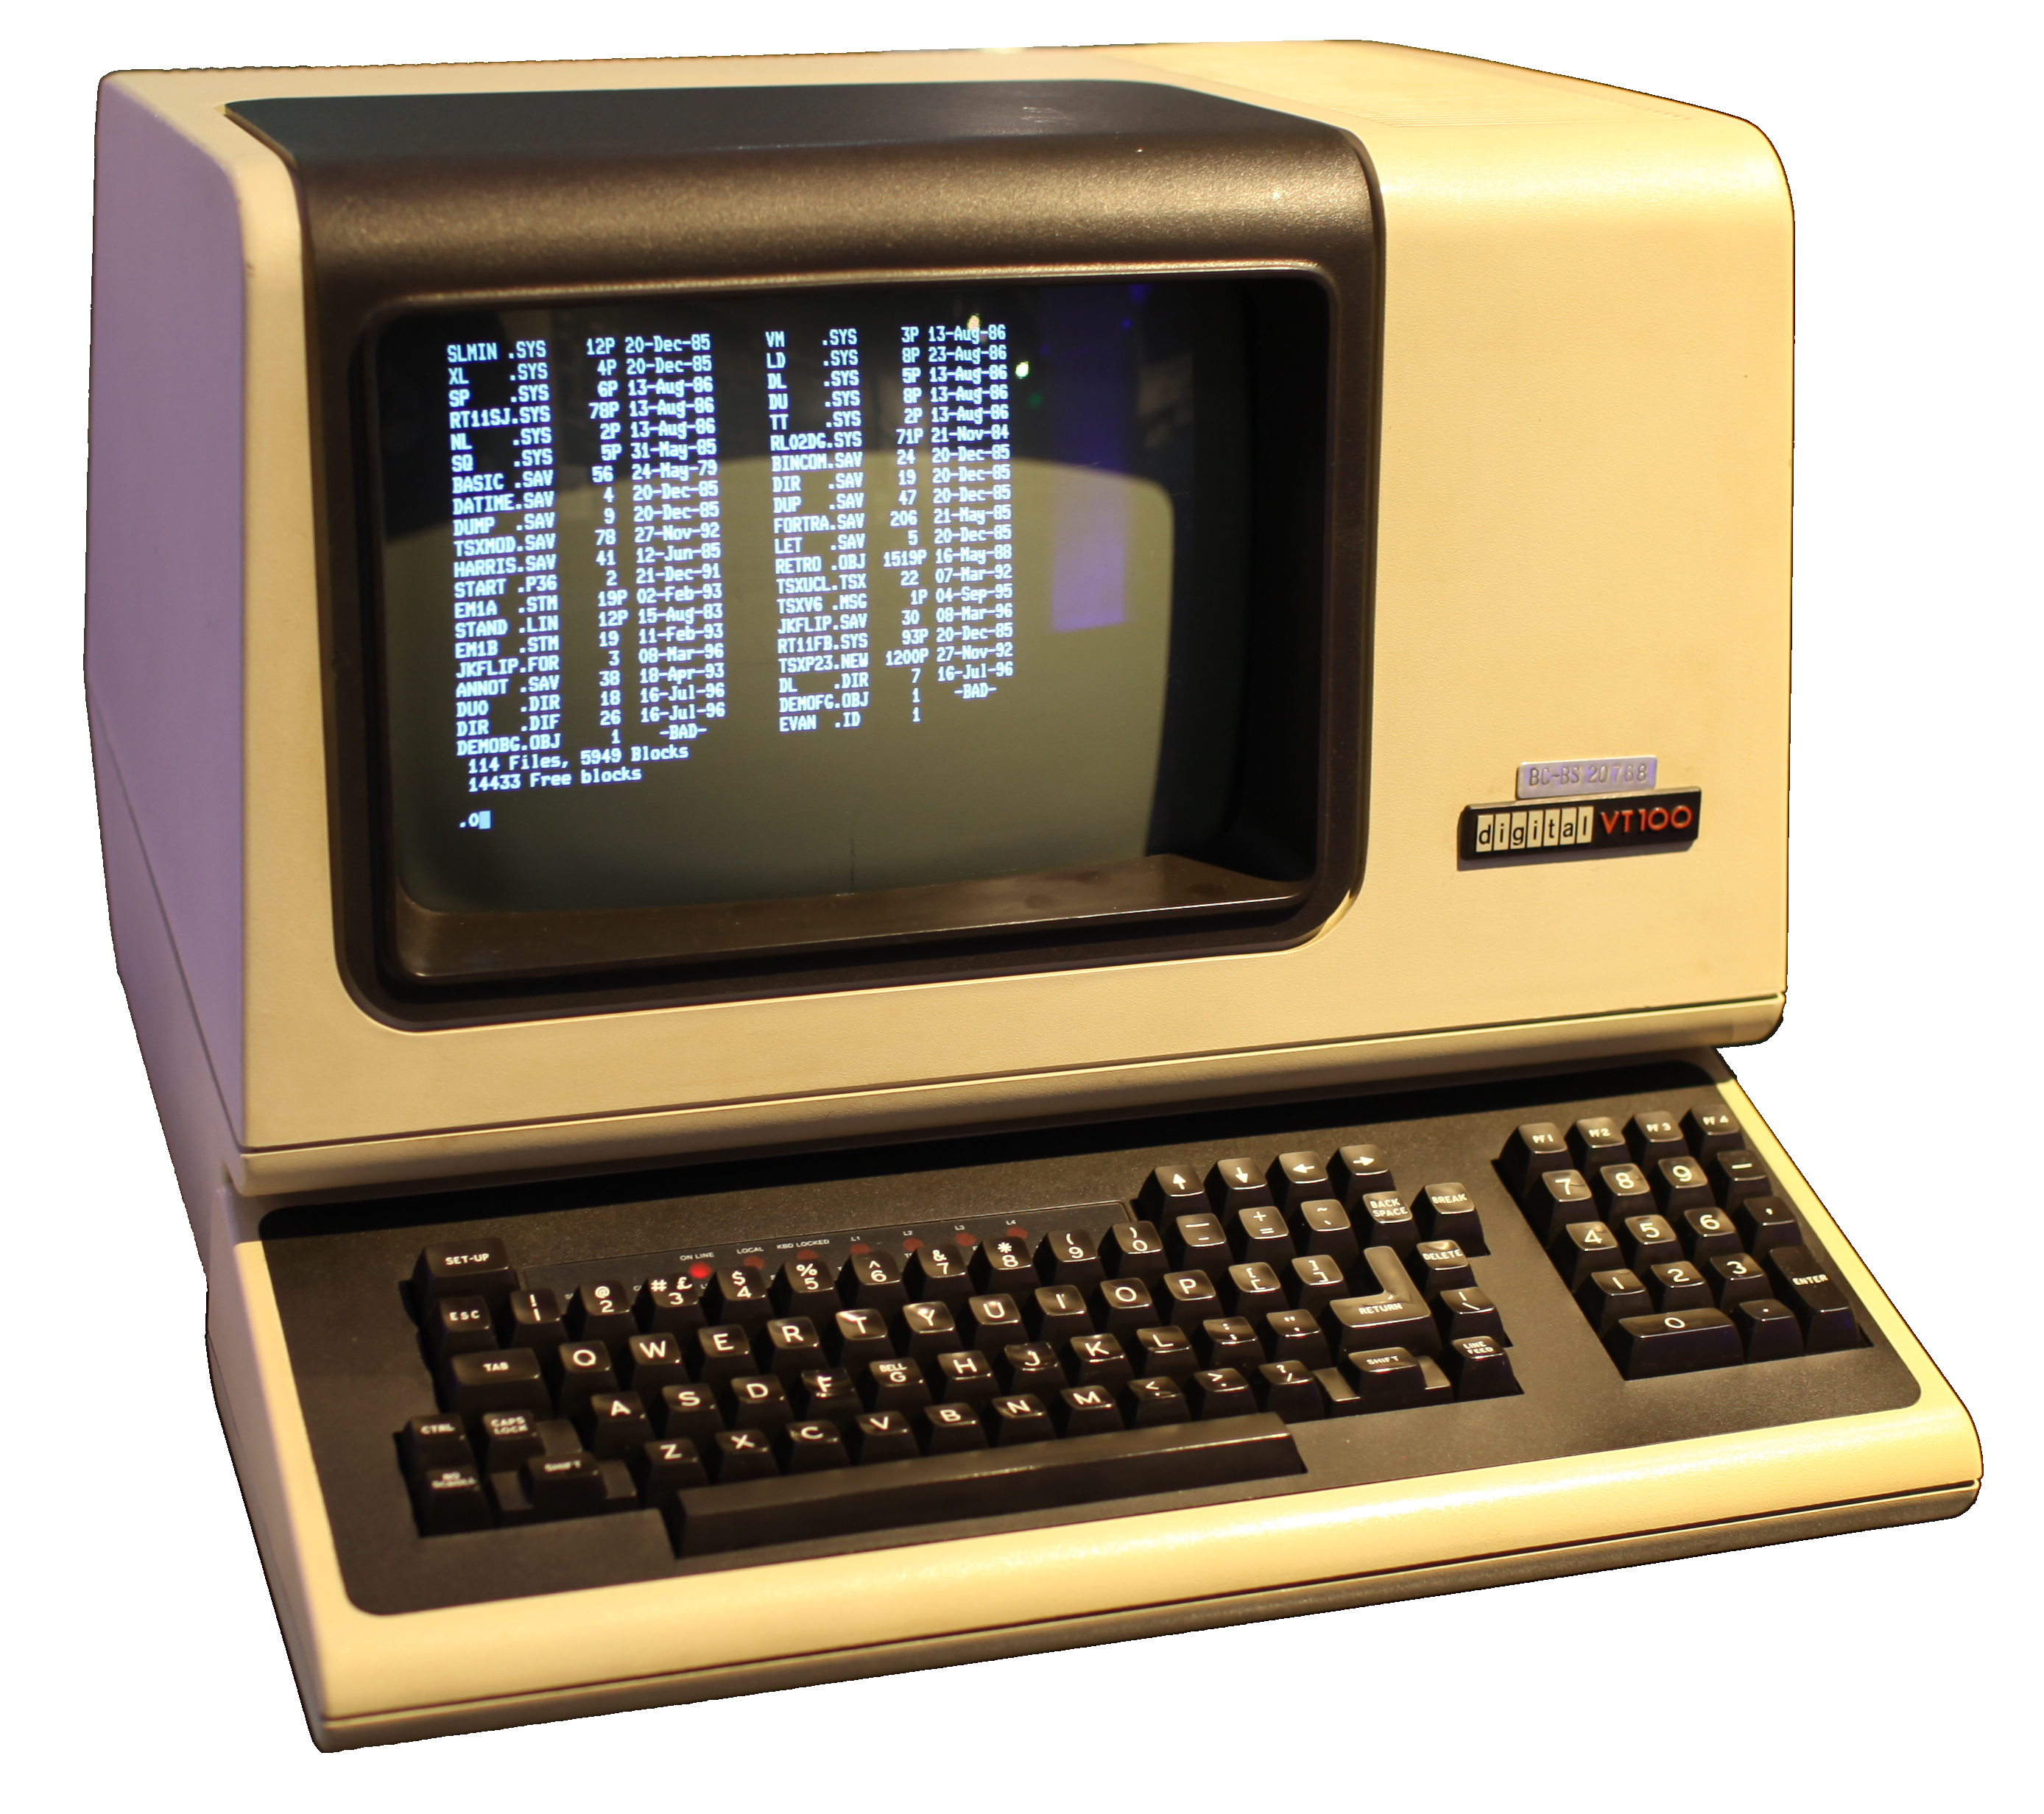
\includegraphics[width=\linewidth]{images/DEC_VT100_terminal_transparent.png}
    \caption{Der VT100 von Digital Equipment Corporation (DEC), gebaut von 1978 bis 1983. (Foto: Gorthmog, \href{https://creativecommons.org/licenses/by-sa/4.0}{CC BY-SA 4.0}, via Wikimedia Commons)}%
    \label{fig:referenz:vt100}
\end{marginfigure}
wurden nicht für moderne Computer erfunden, sondern für Terminals — Bildschirme, die aussahen wie ein Fernseher mit Tastatur und die über eine Leitung mit einem großen Computer verbunden waren. Einer der bekanntesten war der VT100 (siehe Abbildung) von Digital Equipment Corporation (DEC). Auf seinem Bildschirm gab es 24 Zeilen mit je 80 Zeichen — und der Cursor war ein echter, sichtbarer Block, der auf dem Bildschirm stand. Die ANSI-Escapesequenzen, die Ihr heute benutzt, sind die Sprache, mit der man diesen Cursor und den Bildschirm steuert. Moderne Terminals (wie die Konsole auf Eurem Raspberry Pi) verstehen dieselben Sequenzen — sie sind sozusagen die ‚Muttersprache' der Konsole.

Die wichtigsten Sequenzen sind die sogenannten CSI\footnote{%
    CSI steht für ``Control Sequence Introducer'', was so viel wie ``Kontrollsequenzeinführung'' auf deutsch bedeutet.}
Sequenzen -- das CSI steht für \esc{x1B[}, darauf folgen eventuell verschiedene Parameterzeichen (siehe unten) und schließen mit einem Buchstaben, sozusagen dem Kommandocode, ab. 
Ein Beispiel dazu ist \texttt{"\textbackslash x1B[H"}, das Ihr in der Funktion \codeinline{konsole_start} kennengelernt habt. Dabei steht \texttt{H} für das setzen der Cursorposition. Wenn Ihr nun denkt, dann müsste man ja auch die Zeile und Spalte angeben können -- Ihr habt recht, das geht folgendermaßen: \codeinline{printf("\x1B[\%d;\%dH", zeile, spalte);}
Wenn man die Zahlen weglässt, werden also Standardwerte verwendet, in diesem Fall jeweils für Zeile und Spalte die 1.

Es gibt eine ganze Menge an CSI-Sequenzen. Die, die wir in den Beispielen, Programmen, und Übungen verwenden werden -- und auch ein paar mehr, mit denen Ihr vielleicht spielen wollt, zum Beispiel den Farben, sind in den folgenden Tabellen aufgelistet:

\begin{table*}[h]
  \begin{tabular}{cclp{8cm}}
    \toprule
    \textbf{CSI} & \textbf{printf} & \textbf{Name} & \textbf{Effekt} \\
    \midrule
    \texttt{CSI n A}        & \texttt{"\textbackslash x1B[\%dA"}         & Cursor nach oben & 
        Bewegt den Cursor \texttt{n} (Standard ist \texttt{1}) mal nach oben. \\ 
    \texttt{CSI n B}        & \texttt{"\textbackslash x1B[\%dB"}         & Cursor nach unten & 
        Bewegt den Cursor \texttt{n} (Standard ist \texttt{1}) mal nach unten. \\ 
    \texttt{CSI n C}        & \texttt{"\textbackslash x1B[\%dC"}         & Cursor nach rechts & 
        Bewegt den Cursor \texttt{n} (Standard ist \texttt{1}) mal nach rechts. \\ 
    \texttt{CSI n D}        & \texttt{"\textbackslash x1B[\%dD"}         & Cursor nach links & 
        Bewegt den Cursor \texttt{n} (Standard ist \texttt{1}) mal nach links. \\ 
    \texttt{CSI n ; m H}    & \texttt{"\textbackslash x1B[\%d;\%dH"}     & Cursorposition & 
        Bewegt den Cursor in Zeile \texttt{n} und Spalte \texttt{m}. Zeile und Spalte beginnen bei 1, was auch der Standardwert ist, wenn die Zahlen weggelassen werden. \\
    \texttt{CSI n J}        & \texttt{"\textbackslash x1B[\%dJ"}        & Anzeige löschen &
        Löscht Zeichen auf der Konsole: \texttt{0} oder \texttt{1} löschen ab der Cursor-Position alles bis Konsolenende beziehungsweise -anfang. Die \texttt{2} löscht den gesamten Inhalt. \\ 
    \midrule
    \texttt{CSI n m}        & \texttt{"\textbackslash x1B[\%dm"}        & Grafikdarstellung &
        Wählt die Darstellung der Grafik aus. Ist \texttt{n} eine \texttt{0} oder wird weggelassen, werden alle Darstellungsoptionen zurückgesetzt. \\
    \bottomrule
  \end{tabular}
  \caption{Übersicht der ANSI-Escapesequenzen für die Cursor- und Grafiksteuerung.}
  \label{tab:referenz::ansi-esc}
\end{table*}

\newpage\noindent
Außerdem verwenden wir weitere Steuerungscodes, die nicht zum Standard gehören:
\begin{table*}[h]
  \begin{tabular}{cclp{8cm}}
    \toprule
    \textbf{CSI} & \textbf{printf} & \textbf{Name} & \textbf{Effekt} \\
    \midrule
    \texttt{CSI ? 25 h}        & \texttt{"\textbackslash x1B[?25h"}         & Cursor zeigen  & 
        Zeigt den Eingabecursor. \\ 
    \texttt{CSI ? 25 l}        & \texttt{"\textbackslash x1B[?25l"}         & Cursor verstecken &
        Versteckt den Eingabecursor. \\
    \bottomrule
  \end{tabular}
  \caption{Zusätzliche ANSI-Escapesequenzen für die Cursorsteuerung. Diese Sequenzen funktionieren auf fast allen modernen Terminals gehören aber nicht zum ursprünglichen ANSI-Standard.}
  \label{tab:referenz::ansi-esc:extra}
\end{table*}


\vskip5em
\paragraph{Darstellungsoptionen}

\begin{table}[h]
  \centering
  \begin{tabular}{cll}
    \toprule
    \textbf{n} & \textbf{Name} & \textbf{Hinweise} \\
    \midrule
    0 & Normal          & Setzt alle grafischen Optionen zurück. \\
    1 & Fettdruck       & \textbf{Ausgabe mit Fettdruck.} \\
    2 & Gedimmt         & \textcolor{gray}{Verringert die Helligkeit der Schrift.} \\
    3 & Kursiv          & \textit{Kursive (das heißt schräge) Schrift.} \\
    4 & Unterstreichung & \underline{Unterstreichung der Ausgabe.} \\
    7 & Invertierung    & \colorbox{black}{\textcolor{white}{Tauscht die Farben von Vorder- und Hintergrund.}} \\
    30--37 & Vordergrundfarbe & Setzen der Vordergrundfarbe (siehe Tab.~\ref{tab:referenz::ansi-esc:farben}). \\ 
    40--47 & Hintergrundfarbe & Setzen der Hintergrundfarbe. \\
    \bottomrule
  \end{tabular}
  \caption{Liste gebräuchlicher Darstellungsoptionen.}
  \label{tab:referenz::ansi-esc:grafik}
\end{table}

\paragraph{Farben}

\begin{table}[h]
  \centering
  \begin{tabular}{ccc}
    \toprule
    \textbf{Vordergrund} & \textbf{Hintergrund} & \textbf{Farbe (VGA)} \\
    \midrule
    30 & 40 & \cellcolor[RGB]{0,0,0}\textcolor{white}{Schwarz} \\
    31 & 41 & \cellcolor[RGB]{196,0,0}\textcolor{white}{Rot} \\
    32 & 42 & \cellcolor[RGB]{0,196,0}\textcolor{black}{Grün} \\
    33 & 43 & \cellcolor[RGB]{196,126,0}\textcolor{black}{Gelb} \\
    34 & 44 & \cellcolor[RGB]{0,0,196}\textcolor{white}{Blau} \\
    35 & 45 & \cellcolor[RGB]{196,0,196}\textcolor{white}{Magenta} \\
    36 & 46 & \cellcolor[RGB]{0,196,196}\textcolor{black}{Cyan} \\
    37 & 47 & \cellcolor[RGB]{196,196,196}\textcolor{black}{Weiß} \\
    \bottomrule
  \end{tabular}
  \caption{Die klassischen 8 Farben (VGA-Palette).}
  \label{tab:referenz::ansi-esc:farben}
\end{table}

\newpage\chapter{Lösungen zu den Übungen}
\printsolutions

\end{document}
